

\iflong

\begin{frame}
	\frametitle{Applicatons}

	\begin{itemize}
		\item What's a document?
		\item What's a word?
		\item What's your vocabulary?
		\item How do you evaluate?
	\end{itemize}
\end{frame}
\fi

\begin{frame}
\frametitle{Applications}


\begin{block}{
  \only<1>{Computer Vision~\cite{feifei:hdp}}
  \only<2>{Social Networks~\cite{airoldi-08}}
  \only<3>{Music~\cite{hu-09}}
}
\begin{center}
\only<1>{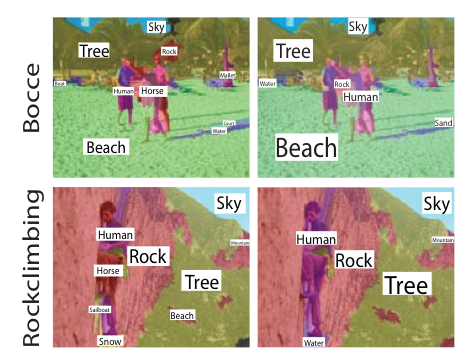
\includegraphics[width=0.8\linewidth]{topic_models/feifei} }
\only<2>{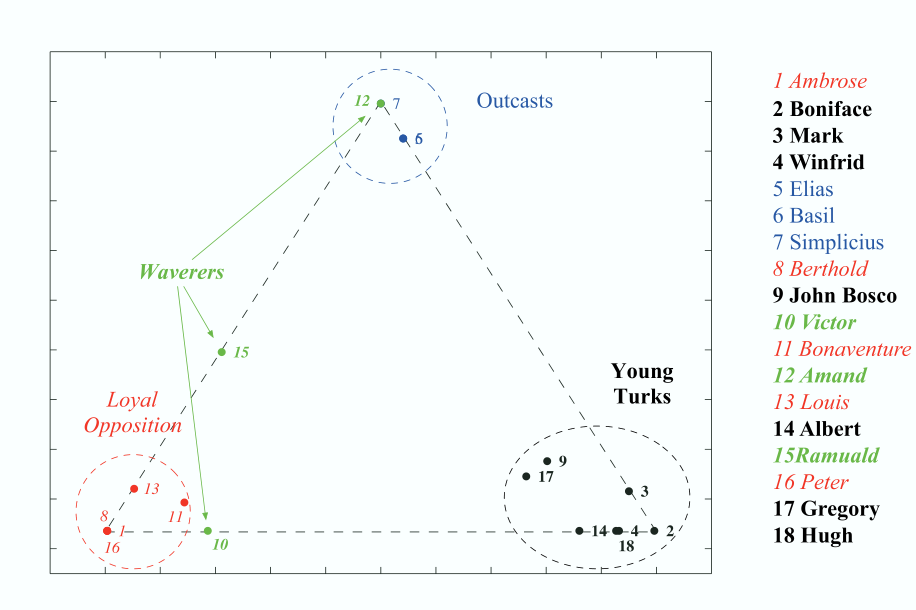
\includegraphics[width=0.8\linewidth]{topic_models/socialnetworks} }
\only<3>{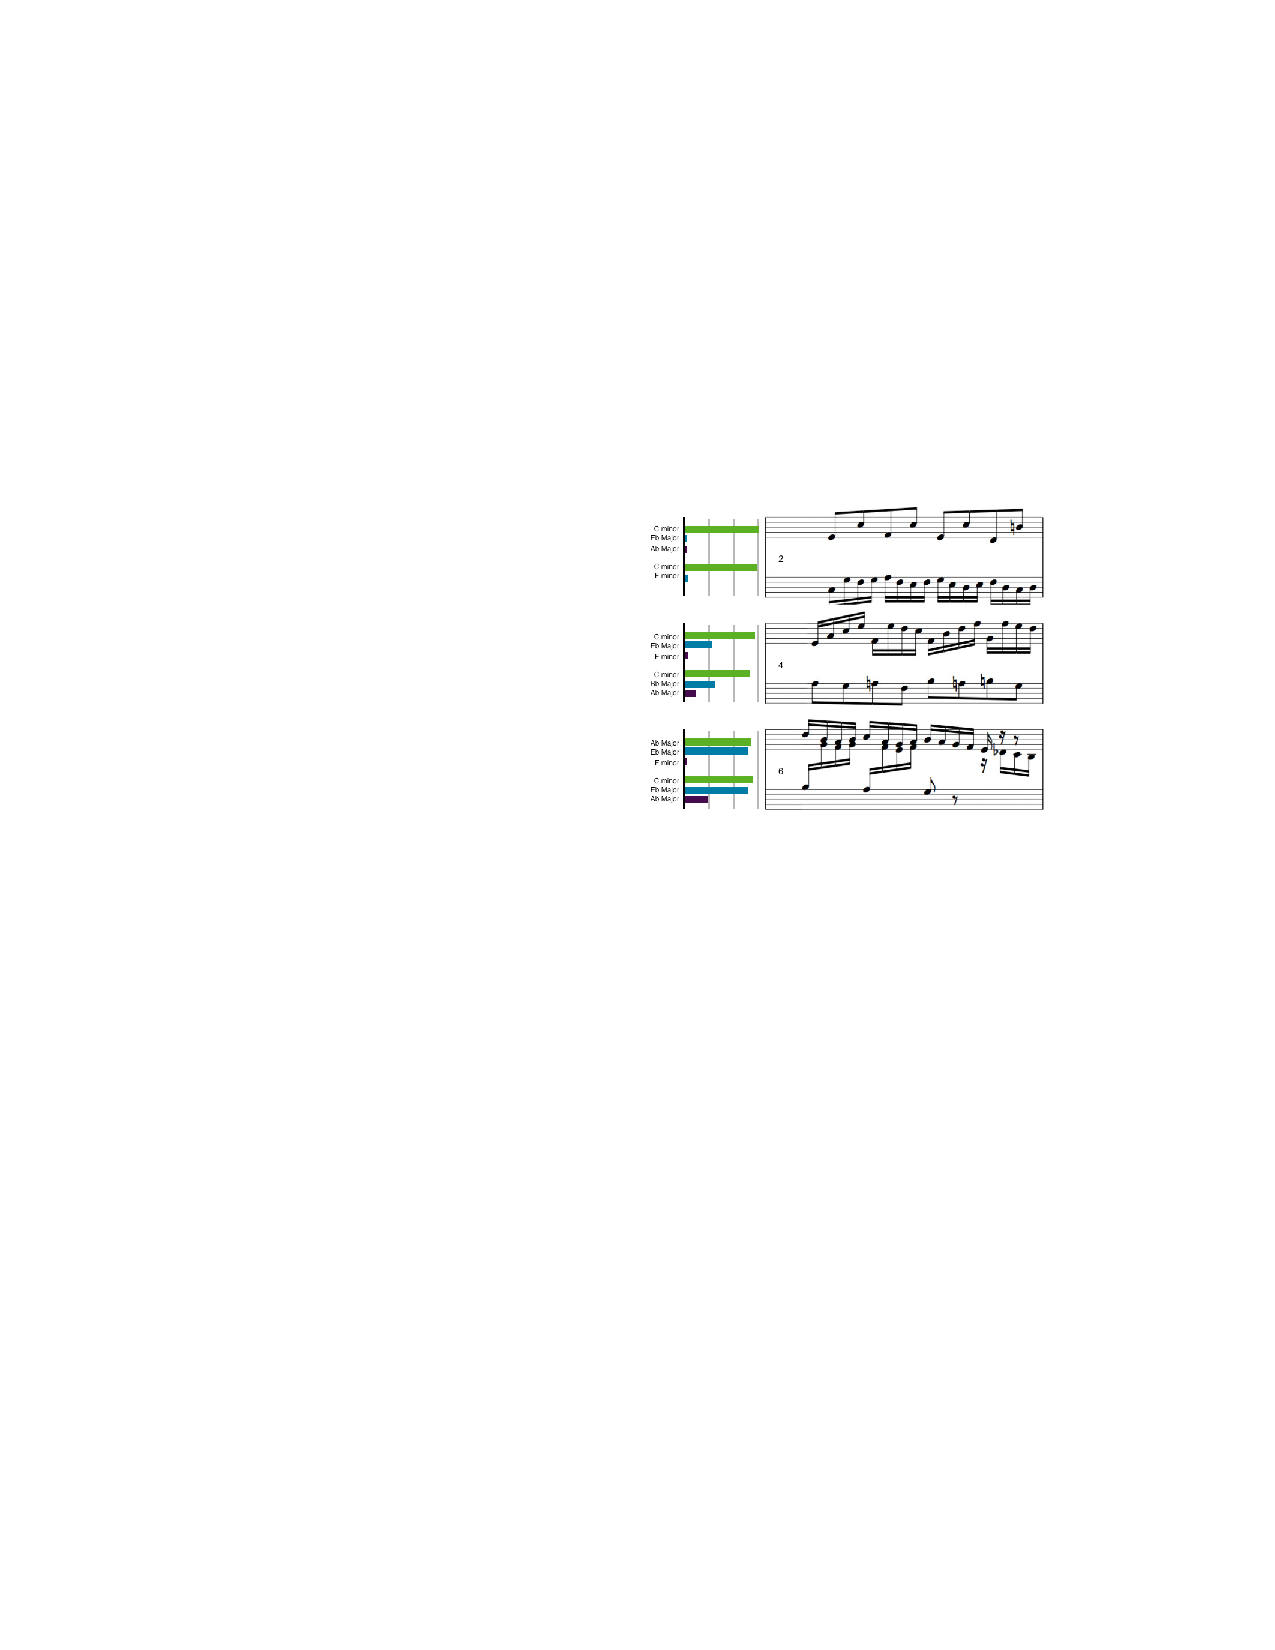
\includegraphics[width=0.8\linewidth]{topic_models/hu} }
\end{center}
\end{block}

\end{frame}

\ifnonpar

\begin{frame}
\frametitle{Nonparametric Models}

\begin{itemize}
\item We've always assumed a fixed number of topics
\item Topic modeling inspired resurgence of nonparametric Bayesian statistics that can handle infinitely many mixture components~\cite{antoniak-74}
\item Equivalent to Rational Model of Categorization~\cite{griffiths-07b}
\item For the rest of this talk, cartoon version - details similar to LDA
\end{itemize}

\end{frame}



\begin{frame}

	\frametitle{Chinese Restaurant Process}

	\begin{itemize}
		\item A process in which $n$ customers sit down in a Chinese restaurant with an infinite number of tables
		\begin{itemize}
			\item First customer sits at first table
			\item $m^{th}$ customer sits at a table drawn from the following distribution given seating history $F$
			\pause
			\begin{align*}
				p(\mbox{previously occupied table } k | F_{m-1}) & \propto n_k \\
				p(\mbox{next unoccupied table} | F_{m-1}) & \propto \alpha
			\end{align*}
		\end{itemize}
	\end{itemize}
\end{frame}

\begin{frame}
	\frametitle{Chinese Restaurant Process}

			\begin{align*}
				p(\mbox{previously occupied table } k | F_{m-1}) & \propto n_k \\
				p(\mbox{next unoccupied table} | F_{m-1}) & \propto \alpha
			\end{align*}

	\begin{itemize}
		\item Defines an exchangeable distribution over partitions of customers
		\item Table assignment corresponds to topic indicator selection $\theta$
		\item Also need to include a topic distribution

\begin{center}
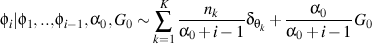
\includegraphics[width=0.8\linewidth]{topic_models/equations/dirichlet_process} \\
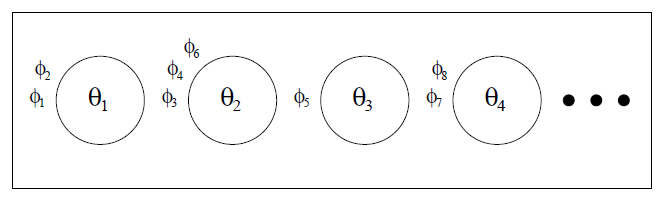
\includegraphics[width=0.7\linewidth]{topic_models/crp}
\end{center}
\end{itemize}

\end{frame}

\begin{frame}
	\frametitle{Chinese Restaurant Franchise}

	\begin{columns}
		\column{0.4\linewidth}
\begin{center}
	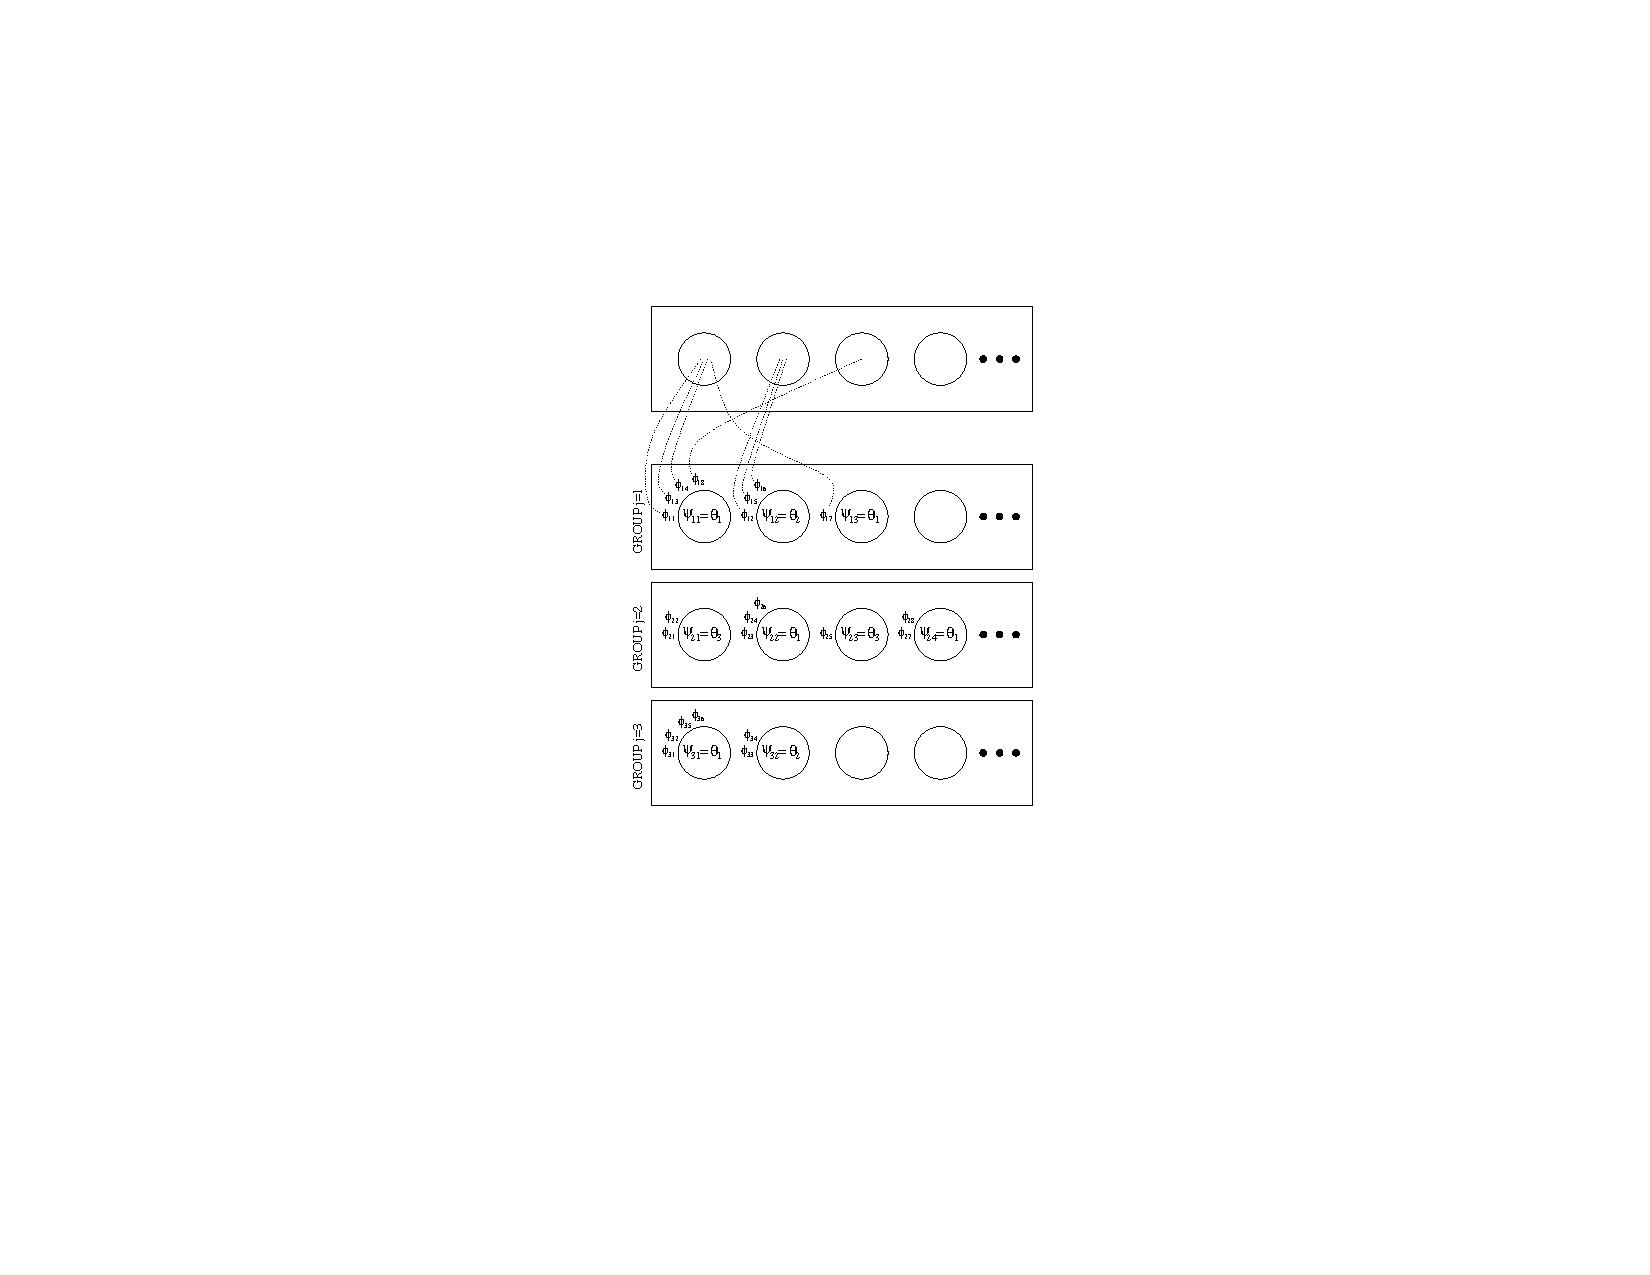
\includegraphics[width=1\linewidth]{topic_models/cr_franchise}
\end{center}

		\column{0.6\linewidth}

	\begin{itemize}
		\item Set of \emph{restaurants} with an unbounded number of \emph{tables} in each restaurant
		\item One \emph{menu} with an unbounded number of \emph{dishes} on the menu
		\item Reinforcement effects: customers sit at popular tables and prefer popular dishes (both globally and locall)
		\item Why?
		\begin{itemize}
			\item Sharing statistical strength: sub-corpora
			\item Consistency across models
			\item Principled backoff\cite{teh-06}
		\end{itemize}
	\end{itemize}

	\end{columns}
\end{frame}

\fi

\iflong

\begin{frame}
	\frametitle{Active research}

	\begin{itemize}
		\item Combining these models with models of syntax
		\item Scaling up to larger corpora
		\item Making topics relevant to social scientists
		\item Humans in the loop
		\item Modeling metadata in document collections
	\end{itemize}
\end{frame}

\fi